% ---------------------------------------------------------------------------
% Section 4: Design. Defines once every term the results use.
% ---------------------------------------------------------------------------

\section{Design}
\label{sec:design}

Every experiment runs the model of \S\ref{sec:model} at the shipped configuration
except where it says otherwise, at one thread, from a committed tree, and writes
each seed's data beside a record of the commit, the full configuration and its
hash, and the library versions. Table~\ref{tab:experiments} lists the
experiments.

\begin{table}[t]
\centering
\small
\begin{tabular}{llrrl}
\hline
Experiment & Question & Seeds & Rounds & Commit \\
\hline
R2-E9 & the transient: four arms, 300 rounds & 40 & 300 & \texttt{349b484} \\
R2-E10 & floor or slow decay: 1000 rounds & 10 & 1000 & \texttt{f4d2b8c} \\
R2-E11 & one-knob sweep, eight cells & 10 & 300 & \texttt{349b484} \\
R2-E13a & training dose: 0.5, 2, 4 passes per round & 10 & 300 & \texttt{f4d2b8c} \\
R2-E13b & exploration slots & 10 & 300 & \texttt{f4d2b8c} \\
R2-E13b-check & comparator check for exploration (post hoc) & 10 & 300 & \texttt{9b11a36} \\
R2-E13c & off-policy ranker & 10 & 300 & \texttt{f4d2b8c} \\
R2-E13d & warm start & 40 & 300 & \texttt{349b484} \\
R2-E14 & open market: replacement & 10 & 600 & \texttt{f4d2b8c} \\
R2-E15 & institutional grid, rounds 250-299 & 10 & 300 & \texttt{f4d2b8c} \\
R2-E15i & institutional slice, inert gate & 10 & 5 & \texttt{f4d2b8c} \\
R2-E15s & institutional grid, rounds 0-4 (post hoc) & 10 & 5 & \texttt{ec0eb83} \\
R2-E16 & floating-point sensitivity, ten runs per seed & 5 & 300 & \texttt{9b11a36} \\
R2-E17 & population size 500 and 2000 & 10 & 300 & \texttt{f4d2b8c} \\
R2-H1r & H1 at the shipped gate, round-0 log & 10 & 1 & \texttt{f4d2b8c} \\
R2-H5r & H5 at the shipped gate & 10 & 40 & \texttt{f4d2b8c} \\
\hline
\end{tabular}

\caption{The experiments, one row per registration, with the commit every seed of
it ran from. Seeds 100--119 are the confirmation set and 42--61 the exploratory set
(\S\ref{sec:design}). Every experiment was registered before it ran except the two
rows marked post hoc; a third post-hoc check, a trend test, needed no new run.
Source: \texttt{data/processed/horizon/run\_index.csv}, built from the per-seed
run records.}
\label{tab:experiments}
\end{table}

\paragraph{Seeds.} There are two sets. The \emph{exploratory} set, seeds 42 to 61,
contains the five seeds every earlier result of this project used. The
\emph{confirmation} set, seeds 100 to 119, took no part in any earlier choice. The
confirmation set is primary and the exploratory set replicates it; experiments
with ten seeds use 100 to 109 and those with five use 100 to 104. A seed fixes a
population (traits, tastes, chemistry, intents and values) and every random
stream downstream of it. The arms of an experiment share each seed's population,
so every comparison is a paired per-seed difference.

\paragraph{Rounds, passes and the margin.} A \emph{round} is one pass of
Algorithm~\ref{alg:round}; a \emph{training pass} is one sweep of the optimizer
over a round's log, about \stepsPerPass{} optimizer steps at the shipped values. Most
experiments run 300 rounds; the floor test runs 1000 and the open market 600. The
\emph{margin} is $0.002$ Gini. A seed's gap is \emph{inside the margin} in a round
when its absolute value is below $0.002$, and the seed's \emph{entry round} is the
first round from which its gap stays inside the margin to the end of the run. A
seed outside the margin at the last round is \emph{censored}. An entry round
differs from the first round a seed is inside the margin whenever the gap
re-crosses the margin after first touching it; only the entry round is used.

\paragraph{Pre-registration.} Each experiment's design, the quantity read, a
prediction with a number in it and a kill condition were committed before the
experiment ran, at commit \texttt{\regCommit} of the repository's
pre-registration file. Three departures are labeled where their results appear:
the primary warm-start measure was fixed after the candidate numbers had been
computed on earlier data (Supplementary note S4), and a comparator check
(\S\ref{sec:what-ends}) and the five-round institutional grid
(\S\ref{sec:institutional}) were added after the registered results were read.
Table~\ref{tab:predictions} lists every registered prediction and whether it
held, scored from the result files by a script rather than by reading.

\paragraph{Statistics.} Intervals are 95\% Student-$t$ intervals over seeds
unless stated. The replicate is the seed, never the round: the rounds of one run
are one trajectory. BCa bootstrap intervals (10{,}000 resamples) accompany the
headline round-99 gap as a check, and at twenty seeds their bounds differ from the
$t$ bounds by at most $\bcaAgree$. Equivalence is tested by two one-sided tests
against $\pm 0.002$ \citep{lakens2017}, whose interval is the 90\% $t$ interval by
construction. Benjamini--Hochberg at $q = 0.05$ corrects the forty cells of the
institutional grid, separately for each comparison arm.

\paragraph{Why one run is not a measurement.} A perturbation of $10^{-7}$ to every
initial weight of the ranker, applied ten times to each of five seeds, leaves the
first rounds unchanged and first moves the gap at round \fpFirstRound. The spread
over a seed's ten runs then grows to $\fpRatioNinetyNine$ of the spread across
twenty seeds at round 99 and to $\fpRatioTwoNinetyNine$ at round 299
(Figure~\ref{fig:fp}). A single run's late-round gap is as much a property of its
floating-point history as of its population. Every number here is therefore a
mean over seeds with an interval over seeds, and every run is at one thread,
because the thread count changes the order of floating-point reductions and so is
part of a run's identity.

\begin{figure}[t]
\centering
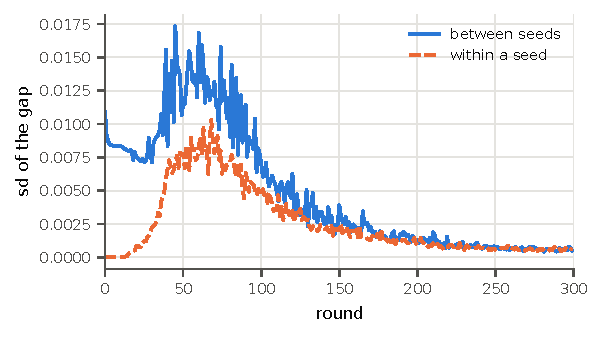
\includegraphics[width=0.62\linewidth]{figures/fp}
\caption{Standard deviation of the gap between seeds (twenty confirmation seeds)
and within a seed (ten runs whose initial weights differ by $10^{-7}$, averaged
over five seeds), by round. Source: \texttt{data/processed/horizon/e16\_fp/} and
\texttt{e09\_canonical/}.}
\label{fig:fp}
\end{figure}

\paragraph{Verification.} Table~\ref{tab:validation} checks the matching and
exposure machinery against results known exactly: the deficit identity that
follows from Hall's theorem under a nested constraint and its Gaussian closed
form, uniqueness of the stable matching under common rankings, the popularity
ranker's closed form, and stability of truncated deferred acceptance on its own
lists. Agreement shows the machinery is correct. It says nothing about whether
the model describes a population.

\begin{table}[t]
\centering
% Generated by paper/tables.py from data/processed/rigor/validation.csv.
% The CSV is written by scripts/run_validation.py and checked against a
% fresh computation by tests/python/test_validation.py.
\resizebox{\textwidth}{!}{%
\begin{tabular}{lllll}
\hline
Check & $N$ & Measured & Evidence & Verdict \\
\hline
Thm 2.2, deficit $D$ & $N=300$ & exact on 5 seeds & matching $=$ empirical sup & agrees \\
Example 2.4 & $N=20{,}000$ & 0.2519 vs $1/4$ & single seed, tol 0.02 & agrees \\
Thm 3.3, $D(14.0)$ & $N=5{,}000$ & 0 & exact & agrees by construction \\
Thm 3.3, $D(30.48)$ & $N=5{,}000$ & 0.7254 & formula 0.7217 & agrees \\
Thm 3.3, unequal var. & $N=5{,}000$ & 0.7433 & formula 0.7380 & agrees \\
Thm 5.1, unique & $N=300$ & same matching both ways & 0 blocking pairs, 5 seeds & agrees \\
Thm 5.1, perturbed & $N=300$ & 22 / 8 / 11 / 12 / 8 pairs differ & uniqueness fails, stability holds & as the theorem requires \\
\hline
\end{tabular}%
}

\caption{Verification against exact results. Rows 1--4: the minimal unmatched
share under a nested compatibility constraint, by exact maximum matching, against
the supremum formula that follows from Hall's theorem \citep{hall1935}, and
against its Gaussian closed form. Rows 5--6: deferred acceptance under common
rankings and under rankings perturbed by 1\% noise \citep{gale1962,knuth1996}.
Row 7: the popularity ranker's exposure Gini against $1 - 2k/N$. Row 8: blocking
pairs of truncated deferred acceptance against its own lists and against full
preferences. Source: \texttt{data/processed/rigor/validation.csv}, written by
\texttt{scripts/run\_validation.py}; a test fails if the file differs from a
fresh computation.}
\label{tab:validation}
\end{table}
